
\medskip

Cet exercice est un questionnaire à choix multiple (QCM).

Pour chaque question, trois réponses (A, B ou C) sont proposées.

\textbf{Une seule réponse est exacte.}

\textbf{Recopier sur la copie} le numéro de la question et la réponse choisie. Aucune justification n'est demandée.

\medskip

\begin{tabularx}{\linewidth}{|m{7cm}|*{3}{>{\centering \arraybackslash}X|}} \hline
	\centering\textbf{Question}& \textbf{Réponse A}& \textbf{Réponse B}& \textbf{Réponse C}\\ \hline
\textbf{1.} Dans une classe de 25 élèves, $60 \%$ des élèves sont des filles.

	Combien y a-t-il de filles dans cette classe ?
	& 10 & 15 & 20 \\ \hline

\textbf{2.} Quelle est la décomposition en produit de facteurs premiers de 126 ?
	& $2 \times 9 \times 7$ & $2^2 \times 5^2 + 2 \times 13$ &$2 \times 3^2 \times 7$ \\ \hline

\textbf{3.} Dans un sac, il y a 17 jetons rouges, 23 jetons jaunes et 20 jetons bleus, tous indiscernables au toucher. On tire au hasard un jeton du sac.

	Quelle est la probabilité d'obtenir un jeton rouge ou un jeton jaune?
	&$\dfrac{2}{3}$ & 0,6 & $\dfrac{17}{23}$  \\ \hline

\textbf{4.} Sur l'octogone régulier ci-dessous, quelle est l'image du segment [DC] par la rotation de centre O qui transforme A en D?

	\hfill~	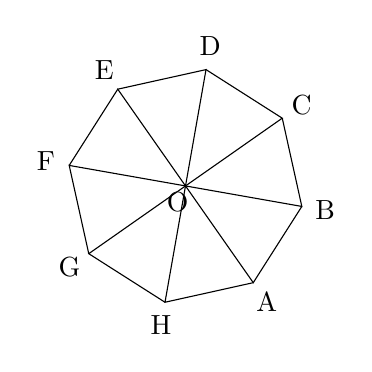
\begin{tikzpicture}[]
		\foreach \a/\n in {1/A, 2/B, 3/C, 4/D, 5/E, 6/F, 7/G, 8/H}
			\draw (0,0)--(-100+45*\a:1.5) node[shift={(-100+45*\a:0.3)}]{\n}--(-55+45*\a:1.5);
		\node at (-0.1,-0.2){O};
	\end{tikzpicture}\hfill~
	& [GE] & [GF] & [AH]\\ \hline

\textbf{5.} Quel est le volume d'un pavé droit de hauteur \np[m]{1,5} et de base rectangulaire de \np[m]{2} de longueur et \np[m]{1,3} de largeur ?

{\small \emph{On rappelle que $\np[m^3]{1}=\np[L]{1000}$.}}
	&\np[m^3]{2,6} & \np[L]{3900}& \np[L]{3000} \\ \hline
\end{tabularx}


\vspace{5mm}
%%%%%%%%
